%-------------------------------------------------------------------
% Document class and package definitions
%-------------------------------------------------------------------
\documentclass[12pt,a4paper,openright,final,twoside]{Essential/cseethesis}

%Included for Gather Purpose only:
%input "thesisreferences.bib"

\begin{document}
%-------------------------------------------------------------------
% Define title, author, etc.
%-------------------------------------------------------------------
\def\thesistitle{Evaluating Post-Quantum Key Exchange in WireGuard }

\def\theauthor{Ludvig Järvi}
\def\theaddress{Dept.\ of Computer Science, Electrical and Space Engineering\\
Lule{\aa} University of Technology\\ Lule{\aa}, Sweden}

\def\supervisors{    Karl Andersson (LTU, Academic Supervisor) \\
    John Lindström (LTU, Academic Supervisor) \\
    Jonas Olson (eCiceron, Internal Supervisor)}
\def\supervisorstring{Supervisors:} % Edit here if you have only one supervisor

% Read abstract and preface from separate files.
% Make sure these exist. See example files.
\def\theabstract{\noindent WireGuard is a widely adopted, modern, free and open-source VPN protocol known for its high performance, minimal codebase, and strong security. Like all VPN protocols relying on classical public-key cryptography, it faces a growing quantum threat in which adversaries are already collecting encrypted traffic today, intending to decrypt it once sufficiently powerful quantum computers become available, a strategy known as ``harvest now, decrypt later''. This thesis evaluates the integration of two NIST-selected post-quantum Key Encapsulation Mechanisms (KEMs): ML-KEM and Hamming Quasi-Cyclic (HQC) into WireGuard's handshake protocol. Both hybrid and pure-KEM handshake variants were designed and implemented in wireguard-go, the official userspace Go implementation of WireGuard, and benchmarked across handshake latency, message size, and per-peer storage requirements. Results show that ML-KEM integrates well as the hybrid ML-KEM-768 variant fits within a single IPv4 packet, adds modest overhead to handshake latency, and keeps storage requirements manageable at scale. Pure ML-KEM variants achieve full post-quantum authentication at the cost of larger messages requiring fragmentation. HQC, by contrast, produces messages large enough to force heavy fragmentation per handshake, resulting in latencies that render it incompatible with WireGuard's design in its current form. The findings suggest that a hybrid ML-KEM-768 deployment is achievable within existing WireGuard infrastructure today, offering protection against harvest now, decrypt later attacks without replacing the current static key infrastructure or causing significant performance degradation. \\

\noindent \textbf{Keywords:} WireGuard, VPN, Post-Quantum, PQ, Post-Quantum Cryptography, PQC, ML-KEM, HQC, Key Encapsulation Mechanism, KEM, Hybrid Cryptography}
\def\thepreface{This thesis would not have been possible without the support and guidance of several people.

I would like to express my sincere gratitude to my supervisors, Karl Andersson, John Lindström and Jonas Olson, for their invaluable feedback, encouragement, and direction throughout this project.

I would also like to thank eCiceron for providing the research context and the resources to explore post-quantum cryptography in a practically motivated setting. 

To my friends and family — thank you for nodding along through many difficult and poorly explained conversations about WireGuard and the looming threat of quantum computers.}


% The definitions above could be put directly in the function call below,
% but is here defined explicitly, for the purpose of clarity.

\startpreamble
  {\thesistitle}
  {\theauthor}
  {\theaddress}
  {\supervisors}
  {\thepreface} 
  {\theabstract}

%% Initialize part containing the thesis introduction chapters
\startchapters
\pagestyle{fancy}

\makeacronyms{\begin{tabular}{ll}
\textbf{AEAD}   & Authenticated Encryption with Associated Data \\
\textbf{CCA}    & Chosen-Ciphertext Attack \\
\textbf{DH}     & Diffie-Hellman \\
\textbf{DoS}    & Denial-of-Service \\
\textbf{ECC}    & Elliptic-Curve Cryptography \\
\textbf{FIPS}   & Federal Information Processing Standards \\
\textbf{FS}     & Forward Secrecy \\
\textbf{HKDF}   & HMAC-based Key Derivation Function \\
\textbf{HNDL}   & Harvest Now, Decrypt Later \\
\textbf{HQC}    & Hamming Quasi-Cyclic \\
\textbf{IP}     & Internet Protocol \\
\textbf{KEM}    & Key Encapsulation Mechanism \\
\textbf{MAC}    & Message Authentication Code \\
\textbf{ML-KEM} & Module-Lattice-based Key Encapsulation Mechanism \\
\textbf{MTU}    & Maximum Transmission Unit \\
\textbf{NIST}   & National Institute of Standards and Technology \\
\textbf{PQ}     & Post-Quantum \\
\textbf{PQC}    & Post-Quantum Cryptography \\
\textbf{PQFS}   & Post-Quantum Forward Secrecy \\
\textbf{PSK}    & Pre-Shared Key \\
\textbf{RKEM}   & Reinforced Key Encapsulation Mechanism \\
\textbf{RSA}    & Rivest-Shamir-Adleman \\
\textbf{RTT}    & Round-Trip Time \\
\textbf{TLS}    & Transport Layer Security \\
\textbf{UAPI}   & Userspace API \\
\textbf{UDP}    & User Datagram Protocol \\
\textbf{VM}     & Virtual Machine \\
\textbf{VPN}    & Virtual Private Network \\
\end{tabular}}

\makechapter[]{Introduction}{Introduction}{Introduction\label{ch1}}
Cryptographic protocols such as Transport Layer Security (TLS), Secure Shell (SSH), and Virtual Private Networks (VPNs) rely on asymmetric cryptography to securely establish shared secrets between previously untrusted parties. These cryptographic systems are based on the assumption that specific mathematical problems, notably integer factorization and discrete logarithms, are too hard for classical computers to solve efficiently.

However, this assumption may not hold in the long term. Rapid advances in quantum computing research suggest that large-scale, fault-tolerant quantum computers may become viable within the coming decades \cite{Swayne2025QuantumRoadmaps}. These are computers capable of leveraging the laws of quantum mechanics to perform quantum algorithms that achieves significant computational speedups for specific classes of problems in comparison to their classical counterparts. Such machines would be able to fundamentally break the asymmetric cryptography primitives used today. 

Two quantum algorithms stand out in this cryptographic context. Peter Shor's algorithm can efficiently factor large integers and compute discrete logarithms \cite{shors}, and Lov Grover's algorithm \cite{grovers}, which provides a quadratic speedup to brute-force key searches. The former directly breaks the public-key primitives underlying RSA, Diffie-Hellman and elliptic-curve cryptography, while the latter reduces the effective security level of symmetric ciphers and hash functions by half.

Once quantum computers reach this critical scale, they will likely be capable of decrypting nearly all historical and contemporary communications secured with current public-key systems. Moreover, adversaries can already capture encrypted traffic today with the intent of decrypting it later when quantum capabilities become available, a strategy commonly referred to as ``harvest now, decrypt later'' \cite{hndl}. This threat makes it essential to begin the transition toward quantum-resistant cryptography as soon as possible, since deploying new cryptographic standards across the Internet ecosystem will take many years.

To stay ahead of this threat, the cryptographic community is actively developing Post-Quantum Cryptography (PQC) algorithms. These are new types of ``quantum-resistant'' mechanisms designed to be secure against both today's computers and tomorrow's quantum machines. The algorithms are based on mathematical problems believed to remain hard for quantum computers, such as those derived from lattices, error-correcting codes, or hash functions. The National Institute of Standards and Technology (NIST) initiated, back in 2016, a global effort to identify and standardize these new methods \cite{nistpqc}, resulting in several promising candidates.

After several years of public evaluation, the NIST Post-Quantum Cryptography Standardization Process selected and standardized ML-KEM \cite{mlkem}, a lattice-based Key-Encapsulation Mechanism (KEM), and is currently in the process of standardizing Hamming Quasi-Cyclic (HQC) \cite{hqc}, a code-based KEM. These schemes are considered primary building blocks for securing Internet communications in the quantum era. 

While the theoretical security of these algorithms has been extensively studied, their practical deployment within real-world communication protocols remains an active research challenge. Post-quantum schemes often have larger key sizes, ciphertexts, and computational overhead compared to classical cryptographic methods. Such differences can significantly affect performance-sensitive protocols that prioritize efficiency.

One such protocol is WireGuard \cite{wireguard}, a modern VPN protocol designed for minimalism, simplicity, and high throughput. WireGuard currently relies on elliptic-curve cryptography, specifically Curve25519, as part of its authenticated key exchange mechanism. While this design offers excellent efficiency on classical hardware, elliptic-curve cryptography is vulnerable to quantum attacks due to its reliance on the discrete logarithm problem.

Integrating PQC into WireGuard therefore presents several unique challenges related to efficiency, compatibility, and code maintainability. These include managing increased message sizes, maintaining low handshake latency, and preserving the protocol's minimalist design philosophy. Existing solutions, such as Rosenpass and PQ-WireGuard prototypes, have demonstrated the feasibility of quantum-resistant VPN connections through external or hybrid key exchanges \cite{rosenpass}\cite{pqwg}\cite{rebar}.

Yet, few studies have systematically compared the performance characteristics of NIST-approved algorithms when integrated into WireGuard's architecture.

This thesis addresses that gap by designing, implementing, and evaluating a hybrid WireGuard handshake that supports two NIST-selected Key-Encapsulation Mechanisms: ML-KEM and Hamming Quasi-Cyclic. The implementation enables an empirical comparison of their latency, computational overhead, memory usage, and message size, and contrasts the results against existing post-quantum WireGuard implementations. By quantifying these trade-offs, the work aims to provide practical insights into the real-world viability of post-quantum VPNs and contribute to the broader effort of securing Internet communications against future quantum threats.

\section{Problem statement and Research Questions}\label{research_questions}
\textit{How does NIST-approved Post-Quantum Key-Encapsulation Mechanisms, specifically ML-KEM and HQC, affect the performance, resource usage, and practical deployability of a post-quantum secure WireGuard handshake compared to existing  approaches?}

\begin{enumerate}[label=\textbf{RQ\arabic*.}]
    \item How do NIST-selected post-quantum key encapsulation mechanisms, specifically ML-KEM and HQC, affect the performance of a WireGuard handshake?

    \item What impact do ML-KEM and HQC have on resource usage in WireGuard, particularly in terms of message size and storage requirements?

    \item To what extent can ML-KEM and HQC be integrated into WireGuard without violating its core design principles, such as low latency and small handshake size?

    \item How do hybrid cryptographic approaches (combining classical Diffie-Hellman with PQC) compare to purely post-quantum approaches in terms of security, performance, and deployability?

    \item How does a hybrid WireGuard implementation using ML-KEM and HQC compare to existing post-quantum solutions in terms of performance and practical deployment?

    \item What trade-offs exist between security level and ciphertext size when selecting PQC algorithms for use in WireGuard?
\end{enumerate}

\section{Scope and Limitations} 
This thesis covers the design, implementation, and empirical evaluation of post-quantum KEM integration into WireGuard's handshake, using ML-KEM and HQC at NIST security levels 3 and 5. The implementation contains both a hybrid mode, which augments the classical handshake with an additional KEM operation, and a pure-KEM mode, which replaces the classical exchange entirely, are implemented and benchmarked. 

Several limitations apply to this work. The implementation is built using \texttt{wireguard-go}, the userspace Go implementation of WireGuard, and does not modify the Linux kernel module. Performance numbers from the kernel implementation would be better due to the absence of TUN interface overhead, so the results here should not be taken as representative of a future kernel-level deployment. 

All benchmarks were conducted on a single hardware platform: two virtual machines running on the same KVM hypervisor. No measurements were taken on physical server hardware, ARM-based processors, or mobile devices.

The benchmark environment uses a virtual network on a single physical host, which eliminates packet loss and real-network jitter. In particular, large handshake messages that exceed the standard MTU are fragmented and reassembled entirely in software, without the reliability problems that IP fragmentation causes on real network paths. Thus, the HQC results in this thesis are measured under more favorable conditions than a real deployment would provide. 

The security analysis of the hybrid and pure-KEM handshake constructions is informal. No formal verification or symbolic proof is provided, and the security arguments in this thesis are based on design reasoning rather than machine-checked proofs. This is consistent with the scope of the related work that this thesis builds on, but it means the security claims are weaker than those of formally analyzed designs.


\section{Thesis Structure} 
The remainder of this thesis is structured as follows.

Chapter 2 provides the necessary background. It begins with classical cryptography, covering classical public-key primitives such as RSA, Diffie-Hellman, and elliptic-curve cryptography, along with key concepts such as key exchange and key encapsulation mechanisms. It then introduces the quantum threat, including a high-level overview of quantum computing and the algorithms that break classical cryptography: Shor's and Grover's algorithms, as well as the ``harvest now, decrypt later'' risk model. Finally, it introduces post-quantum cryptography, covering the main algorithm families with a focus on ML-KEM and HQC, and discusses hybrid cryptographic approaches and the practical challenges of deploying PQC in real protocols. 

Chapter 3 covers the WireGuard protocol. It describes its design principles, the Noise Protocol Framework, the IKpsk2 handshake pattern, the cryptographic primitives in use, the full handshake flow, and the Go implementation. It also discusses the specific challenges that arise when integrating post-quantum algorithms into WireGuard. 

Chapter 4 discusses the related work on post-quantum WireGuard, covering the original PQ-WireGuard by Hülsing et al., the Rosenpass sidecar approach, and the recent Rebar redesign using reinforced KEMs by Hashimoto et al. It also describes concurrent work, covering the ongoing NIST standardization of HQC and the deployment of hybrid ML-KEM in TLS 1.3.

Chapter 5 describes the research method. It covers the literature study, protocol analysis, design decisions, implementation of both the hybrid and pure-KEM handshake variants, measurement methodology, and benchmarking setup. It concludes with a discussion of reliability, validity, and generalizability. 

Chapter 6 presents the results of the benchmark: handshake latency, message sizes, and storage requirements for all nine evaluated variants, compares them against the related work, and describes how they answer the research questions. 

Chapter 7 outlines the contributions of the thesis to literature, practice, and management, examines the MTU constraint in detail, addresses the requirements of full post-quantum authentication, and compares the implementation with PQ-WireGuard, Rosenpass, and Rebar. It also considers the ethical and sustainability implications of the transition to post-quantum cryptography, and aims to direct future research.

Chapter 8 concludes the thesis by summarising the main findings and reflecting on the broader implications for post-quantum VPN deployment.

\makechapter[]{Background}{Background}{Background\label{ch2}}
\section{Asymmetric Cryptography}
Asymmetric cryptography, also referred to as public-key cryptography, addresses the fundamental problem of symmetric cryptography in secure communications: how can two previously unknown parties establish a secure channel without first meeting up in person to exchange a secret key. 

In order to solve this problem, asymmetric cryptography uses two mathematically related keys: a private key and a public key. The public key can be distributed freely, while the private key must remain secret. Messages encrypted with a public key can then only be decrypted using its corresponding private key, enabling secure communications without the need for a predetermined shared secret.

To demonstrate this concept, imagine two people: Alice and Bob. Alice wants to send a secret message to Bob. To achieve this, they do the following: 
\begin{enumerate}
    \item Bob sends a box and an open padlock, to which only Bob has the key, to Alice.
    \item Alice places her message in the box, locks it with the padlock, and sends it back to Bob.
    \item Bob uses his key to unlock the box and is able to read Alice's message.
\end{enumerate}
Even if some adversary were to intercept the box on its way back to Bob, they would be unable to open it and read Alice's message since they don't have Bob's key.

This analogy describes the core idea of asymmetric cryptography: separating the methods of encryption and decryption. Here the padlock represents the public key, and Bob's key the private key. He can send copies of his padlock to anyone who wants to send him a secret message, knowing only he can open them.

In practice, these systems use specific mathematical problems known as trapdoor functions \cite{trapdoor}. These are problems that are easy to compute in one direction, but computationally infeasible to reverse without hidden information (the private key).

Asymmetric cryptography is not used directly to encrypt large amounts of data due to its computational overhead. Instead, it is commonly used during the initial handshake phase of a protocol to establish a shared symmetric key. Once this shared secret has been established, symmetric encryption algorithms can be used to protect the bulk of the communication efficiently.

\subsection{RSA and Diffie-Hellman}
The first generation of widely adopted asymmetric systems relied on two primary mathematical hurdles. The RSA (Rivest-Shamir-Adleman) algorithm, introduced in 1977 by Ron Rivest, Adi Shamir, and Leonard Adleman \cite{rsa}, built on the mathematical difficulty of factoring large composite integers. While multiplying two large prime numbers is computationally trivial, determining the original factors from their product is believed to be infeasible for sufficiently large numbers using classical algorithms. This asymmetry forms the mathematical foundation of the RSA algorithm.

The other fundamental primitive introduced to public-key cryptography was the Diffie-Hellman (DH) key exchange, introduced in 1976 by Whitfield Diffie and Martin Hellman \cite{dh}. Rather than encrypting messages directly, Diffie-Hellman introduced the concept of a secure key exchange, enabling two parties to establish a shared secret over an insecure channel without ever transmitting the secret itself. As illustrated in Figure \ref{fig:DH}, each party generates a private key and exchanges a corresponding public key derived from it. Both parties can then independently compute the same shared secret from the other's public key and their own private key. The security of this protocol relies on the hardness of the discrete logarithm problem, which states that recovering the private exponent from the public key alone is computationally infeasible.

\begin{figure}[H]
\centering
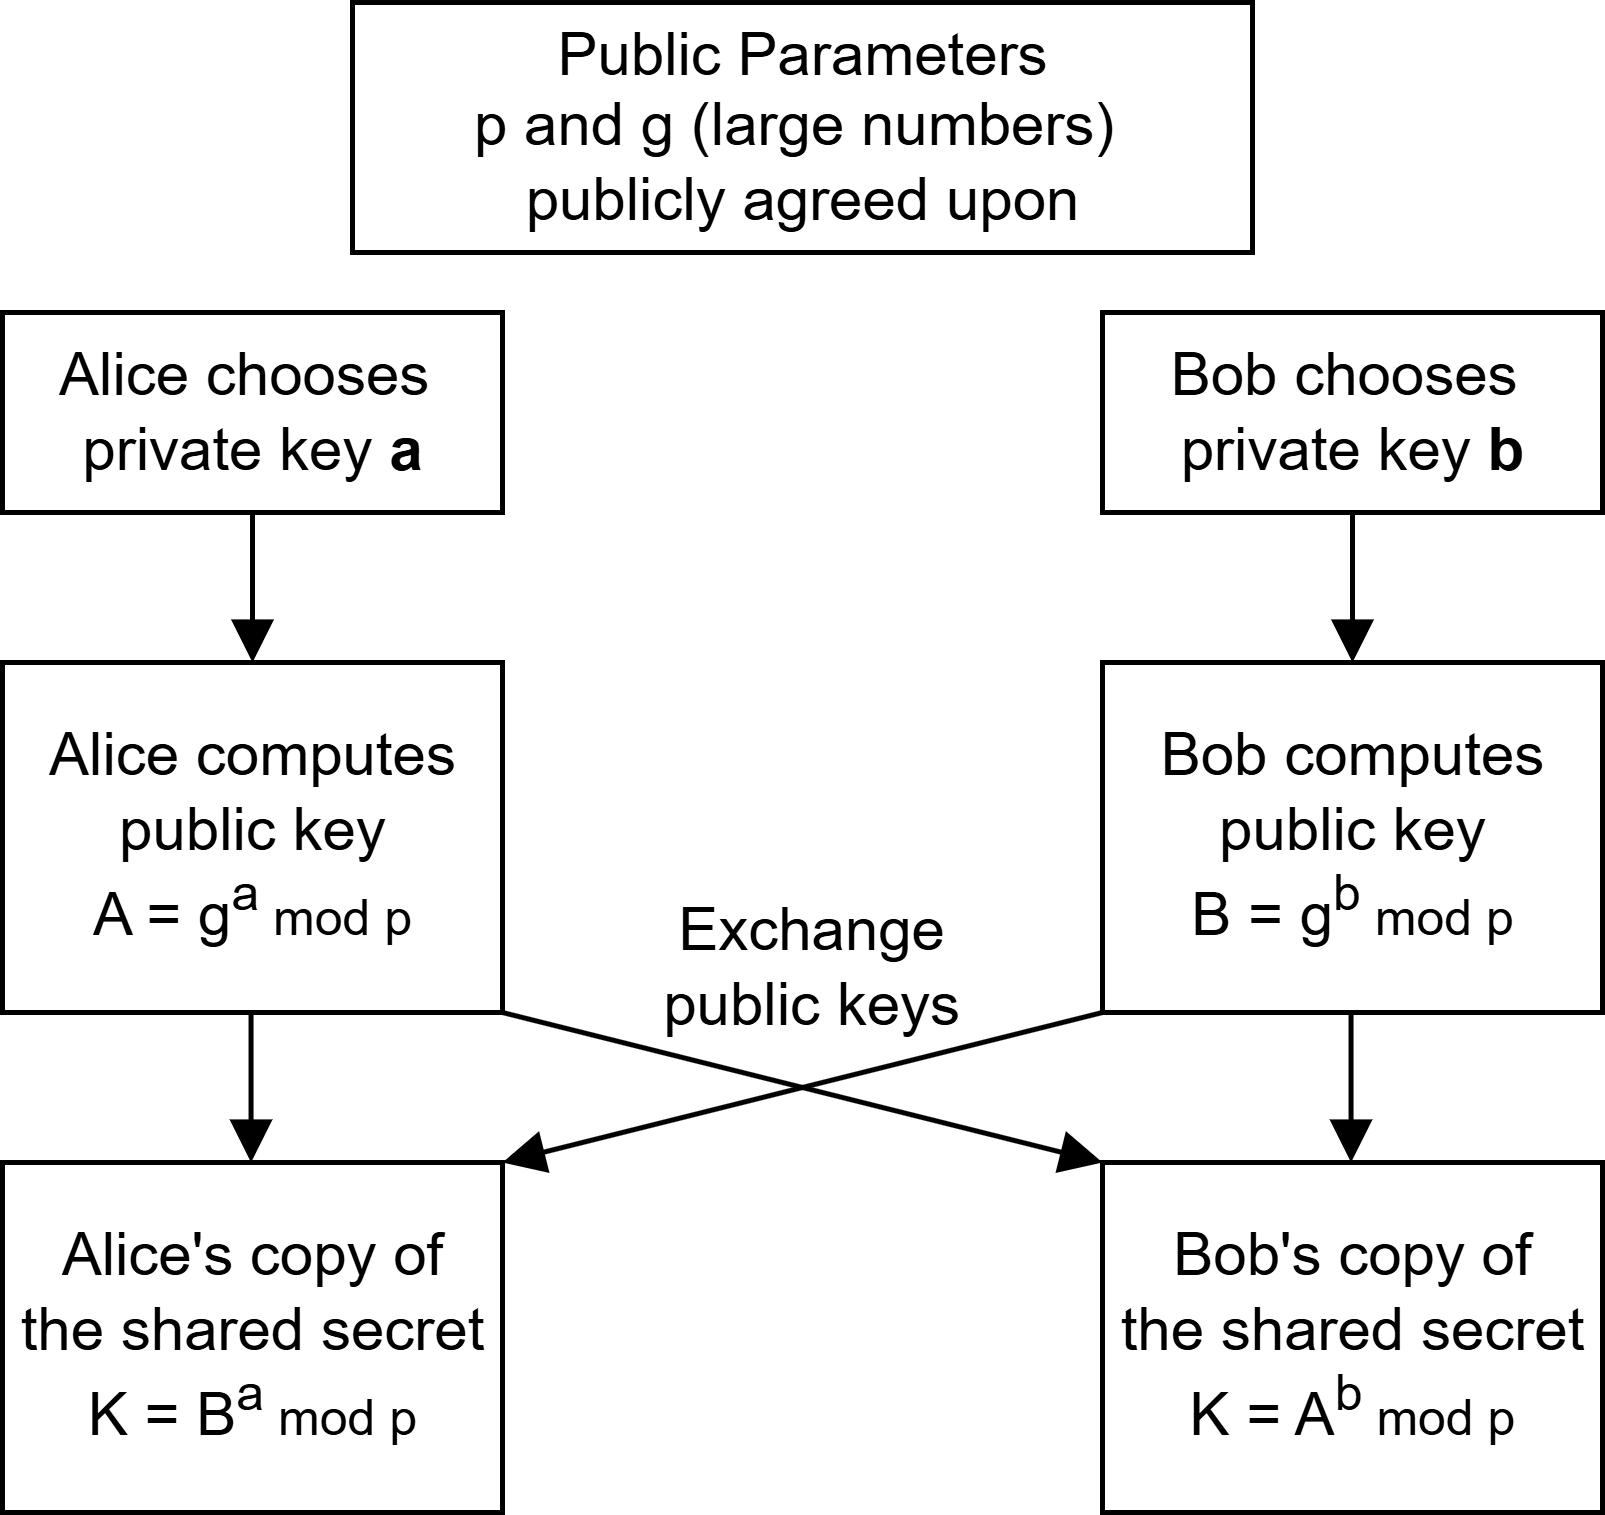
\includegraphics[width=0.8\textwidth]{Images/dh.png}
\caption{A simple view of key establishment using Diffie-Hellman.}
\label{fig:DH}
\end{figure}

These methods defined the first thirty years of digital security, but as computational power grew, the required key sizes for RSA and standard DH became unmanageable, leading to a need for more efficient mathematics.

\subsection{The Shift to Elliptic-Curve Cryptography}
In the early 2000s, many cryptographic protocols began transitioning toward Elliptic-Curve Cryptography (ECC). Instead of operating over finite fields of integers, ECC relies on the algebraic structure of elliptic curves over finite fields. The advantage of the Elliptic Curve Discrete Logarithm Problem (ECDLP) is that it is significantly harder to solve per bit of key size than the two previous mathematical problems that RSA and DH are based on.

For example, a 256-bit elliptic curve key, such as Curve25519 used by WireGuard, provides a security level equivalent to a 3072-bit RSA or DH key \cite{Barker}. This efficiency is one of the primary reasons modern protocols have adopted ECC. Smaller key sizes reduce bandwidth requirements and computational overhead, enabling faster handshakes and smaller packet headers, which are particularly important for performance-sensitive systems such as VPN protocols.

Despite their efficiency, elliptic-curve systems remain fundamentally vulnerable to quantum attacks due to their reliance on discrete logarithm problems. This vulnerability forms one of the key motivations for the development of post-quantum cryptographic algorithms. Recognizing this risk, NIST has initiated a long-term transition toward quantum-resistant cryptographic algorithms. Current guidance recommends that organizations begin migrating away from classical public-key mechanisms in the coming years, with many traditional systems expected to be phased out after approximately 2030 as post-quantum standards are deployed \cite{PQCTransition}. Such a transition highlights the need to evaluate how existing protocols that rely heavily on elliptic-curve cryptography, such as WireGuard, can adapt to post-quantum cryptographic primitives.

\subsection{Key Exchange vs. Key Encapsulation}
It's important to distinguish between the two main methods for establishing shared symmetric cryptographic keys. 

Traditional key exchange protocols such as Diffie-Hellman employ an interactive process in which both parties contribute to the generation of a shared secret. Instead of sending the secret directly, each party exchanges intermediate values derived from their private key, and both participants can independently compute the same shared key from the other's public value. This bidirectional structure is displayed in Figure \ref{fig:DH}.

In contrast, asymmetric post-quantum algorithms including ML-KEM and HQC are designed as Key Encapsulation Mechanisms (KEMs). Rather than a mutual exchange, KEMs follow a sender-receiver model. As shown in Figure \ref{fig:KEM}, the sender runs the encapsulation algorithm using the recipient's public encapsulation key, producing both a ciphertext and a shared secret. The ciphertext is transmitted to the recipient, who uses their corresponding private decapsulation key to run the decapsulation algorithm and recover the same shared secret. No interactive contribution from the recipient is required.

\begin{figure}[H]
\centering
\includegraphics[width=0.8\textwidth]{Images/kem.png}
\caption{A simple view of key establishment using a KEM}
\label{fig:KEM}
\end{figure}

While the end result is the same, both parties arrive at a shared secret, the logistical flow is different. This distinction is a core challenge when integrating post-quantum KEMs into existing protocols like WireGuard, which was originally designed for the interactive key exchange flow of Diffie-Hellman. 

Despite this difference in their structure, KEMs are the flow used for post-quantum cryptography due to the nature of the mathematical problems on which post-quantum security is based. These do not support the bidirectional structure of a key exchange protocol. Instead, they lend themselves to a one-directional approach where one party can efficiently encapsulate a secret under a public key, while only the holder of the corresponding private key can recover it.


\section{The Quantum Threat}
As discussed in the introduction, the long-term security of modern cryptographic systems relies on the assumption that certain mathematical problems are computationally infeasible for classical computers to solve. However, the development of quantum computing challenges this assumption. Quantum computers operate according to the principles of quantum mechanics and are capable of executing algorithms that can outperform classical algorithms for specific types of problems. 

There are two quantum algorithms that are especially relevant in this context: Shor's algorithm, which efficiently solves integer factorization and the discrete logarithm problem, and Grover's algorithm, which accelerates brute-force search. These algorithms are the frontrunners of the quantum threat to current cryptographic systems and are discussed in the following sections.

\subsection{Quantum Computing}
We must establish a high-level understanding of how quantum computers work in order to understand how they are able to threaten current encryption. 

A classical computer processes information using bits, binary values that exist in one of two states: 0 or 1. These bits are manipulated deterministically through electrical circuits made up of transistors and logic gates, which enables the computer to perform arithmetic and logical operations. At any given point in time, a classical system represents a single, well-defined state.

A quantum computer instead operates using quantum bits, commonly referred to as \textit{qubits}, which has the ability to exist in a superposition of both states simultaneously. As a result, a qubit represents a linear combination of the two states rather than a single deterministic value. When multiple qubits are combined, the system can represent a probability distribution of many possible states at once. For a system of $n$ qubits, this corresponds to $2^n$ possible configurations, resulting in an exponentially large state space.

The other key property of quantum systems is entanglement, where the states of multiple qubits become correlated in a way such that the state of one qubit cannot be described independently of the others. Entanglement enables quantum computers to capture and exploit relationships between variables in ways that are not possible in classical systems.

Quantum algorithms leverage superposition, entanglement, and the manipulation of probability amplitudes to perform certain classes of computations in a fundamentally different way than classical algorithms. By carefully controlling how probability amplitudes evolve during computation, these algorithms can amplify the likelihood of correct solutions while cancelling out incorrect ones. This interference structure is what enables quantum computers to achieve significant speedups over classical computation for problem classes where it can be meaningfully exploited \cite{Brassard2000Amplitude}.

\subsection{Shor's Algorithm}
One of the most significant breakthroughs in quantum computing for cryptography was the discovery of Shor's algorithm by Peter Shor in 1994 \cite{shors}. The algorithm provides an efficient quantum method for solving the two mathematical problems that are central to modern public-key cryptography: integer factorization and the discrete logarithm problem.

In order to fully grasp the impact of Shor's algorithm, let's first consider the best known classical algorithm for solving these problems. The General Number Field Sieve (GNFS) operates in sub-exponential but superpolynomial time \cite{GNFS}, which means that every additional digit in an integer makes the factorization time disproportionately longer. While significantly faster than naive approaches, the computational cost still grows at an infeasible rate for larger key sizes. The largest RSA integer factored to date is RSA-250, an 829-bit number factored in February 2020 using CADO-NFS, an optimized software implementation of GNFS \cite{CADO-NFS}. This required approximately \num{2,700} CPU core-years \cite{RSA250}, illustrating that classical factoring remains computationally prohibitive at the key sizes used in practice.

Shor's algorithm completely demolishes this notion of infeasibility. By leveraging the principles of quantum mechanics, it is able to factor large integers and solve discrete logarithms in polynomial time. It accomplishes this by reducing the problem into a period-finding problem. Given an integer $N$, the algorithm selects a random value and constructs a function whose period is related to the factors of $N$. While finding such periods is computationally difficult for classical computers, quantum computers can solve this efficiently using the Quantum Fourier Transform (QFT).

The practical implications of Shor's algorithm have been extensively explored and optimized in later research. A widely cited paper by Craig Gidney and Martin Ekerå demonstrated in 2021 that factoring a 2048-bit RSA integer could be feasible using a quantum computer with around 20 million physical qubits and 8 hours of computation time, assuming realistic error rates, cycle times and reaction times \cite{Gidney2021RSA2048}. This paper has recently received a follow-up by Gidney alone where he demonstrated that the same task could accomplished in less than a week using less than a million noisy qubits under the same assumed constraints \cite{Gidney2025RSA2048}.

Thus, the existence of Shor's algorithm represents a fundamental threat to modern public-key cryptography. Since protocols such as TLS, SSH, and VPN systems rely on RSA, Diffie-Hellman, or elliptic-curve cryptography for secure key establishment, the availability of large-scale quantum computers would render these systems insecure.

\subsection{Grover's Algorithm}
Grover's algorithm \cite{grovers} addresses a different class of problems than Shor's algorithm, specifically unstructured search. Given a search space of size $N$, a classical brute-force algorithm requires $\mathcal{O}(N)$ evaluations to find a target element. Grover's algorithm reduces this complexity to $\mathcal{O}(\sqrt{N})$ by leveraging quantum amplitude amplification.

In the context of cryptography, Grover's algorithm impacts symmetric-key primitives such as block ciphers and hash functions. But, unlike Shor's algorithm, Grover's algorithm does not completely break symmetric cryptographic schemes. Instead, it effectively halves their security level in terms of bit strength. This degradation can be mitigated by increasing key sizes. For example, a 128-bit symmetric key, which is considered secure against classical adversaries, would offer only 64 bits of security against a quantum adversary using Grover's algorithm. Consequently, doubling the key length (from 128 to 256 bits) is generally considered sufficient to maintain security in a post-quantum setting.

It is also important to note that practical implementations of Grover's algorithm face significant overhead due to error correction and circuit depth requirements, which further limits its near-term applicability. But it remains a critical consideration when evaluating the long-term security of symmetric cryptographic systems.

\subsection{``Harvest now, decrypt later.''} \label{hndl}
A common misconception about the quantum threat is that it only becomes relevant when sufficiently large quantum computers become available, but this view overlooks an already active risk model known as ``harvest now, decrypt later'' (HNDL) \cite{hndl}.

In this model, an adversary intercepts and stores encrypted communication today with the intention of decrypting them in the future once sufficiently powerful quantum computers exist. This strategy is particularly concerning for data with long-term confidentiality requirements, such as government communications, intellectual property, personal data, and critical infrastructure information. 

It is important to understand what part of modern encrypted communication is vulnerable in this context. While data at rest is protected by symmetric encryption algorithms such as AES, which are considered resistant to quantum attacks, the asymmetric public-key algorithms used during the key exchange are the primary target. If an adversary can intercept the key exchange step of a session protected by TLS for example, they can store it and later use a quantum computer to recover the symmetric session key and decrypt all the session data. The implication is that even data which appears to be well-protected at rest may be vulnerable if the key exchange that established its protection was recorded.

The HNDL threat has driven significant regulatory action across multiple jurisdictions, each establishing strict timelines for the transition to post-quantum cryptography directly motivated by HNDL risk.  

In the United States, the NSA's Commercial National Security Algorithm Suite 2.0 (CNSA 2.0) establishes a phased migration schedule for National Security Systems. Traditional networking equipment such as VPNs and routers is required to support and prefer CNSA 2.0 algorithms by 2026, and to use them exclusively by 2030. Large-scale public-key infrastructure systems, such as TLS, follow a slightly later schedule, with mandatory preference by 2030 and exclusive use by 2033 \cite{NSA2022CNSA2}. 

In Europe, the European Commission published a coordinated PQC implementation roadmap, which establishes a timeline for the transition to PQC for all member states. Under this roadmap, all member states are expected to have begun transitioning to post-quantum cryptography by the end of 2026, with critical infrastructure systems fully transitioned to PQC no later than the end of 2030 \cite{EUPQC2025Roadmap}.

At the standards level, NIST's deprecation timelines add further urgency. Classical quantum-vulnerable algorithms providing less than 128 bits of security are set to be deprecated after 2030 and disallowed after 2035, with algorithms above the 128-bit level set to follow the same eventual prohibition \cite{Moody2025PQCRoadAhead}.

The ``harvest now, decrypt later'' threat establishes that the urgency of post-quantum migration is determined not only by the arrival of quantum computers, but also by the confidentiality requirements of data being transmitted and stored today. The combination of already-active data collection, long cryptographic migration timelines, and firm regulatory deadlines means that organizations handling sensitive data must treat the transition to quantum-resistant cryptography as an active and ongoing priority.


\section{Post-Quantum Cryptography}
Post-Quantum Cryptography (PQC) refers to cryptographic algorithms that are designed to remain secure against attacks from both classical and quantum computers. The goal is to replace or complement current cryptographic primitives such as RSA, Diffie-Hellman, and ECC. In many cases, PQC schemes are designed to be integrated into existing protocols with minimal changes, although this still requires adaptations due to fundamental differences in protocol logic and accommodation for larger key sizes.

PQC algorithms are based on mathematical problems that are believed to be hard even for quantum computers. The main categories include lattice-based, code-based, multivariate, and hash-based cryptography. This thesis focuses on the two NIST-selected approaches: lattice-based cryptography (ML-KEM) and code-based cryptography (HQC).

\subsection{Lattice-Based Cryptography (ML-KEM)}
ML-KEM (Module-Lattice-Based Key-Encapsulation Mechanism), formerly known as CRYSTALS-Kyber \cite{kyber}, is a lattice-based KEM standardized by NIST in Federal Information Processing Standards (FIPS) publication 203 \cite{mlkem} in August 2024.

ML-KEM is based on the hardness of lattice problems, specifically the so-called Module Learning With Errors (MLWE) problem. The core idea is that a system of linear equations with small random errors is computationally hard to solve, even for a quantum computer.

One of the main advantages of ML-KEM is its strong performance and relatively moderate key sizes when compared to other PQC candidates. For example, ML-KEM-768 has a public key size of around \qty{1184}{bytes}, which is manageable in protocols like TLS. Key generation and encapsulation are also significantly faster than RSA. These properties make ML-KEM suitable for practical deployment, which is why NIST selected it as the primary standard for post-quantum key establishment.

\subsection{Code-Based Cryptography (Hamming Quasi-Cyclic)}
Hamming Quasi-Cyclic (HQC) \cite{hqc} is a code-based KEM selected by NIST in March 2025 as a backup standard to ML-KEM \cite{Moody2025NISTIR8545}. A draft standard is expected in 2026, with finalization planned for 2027.

The security of HQC is based on the hardness of decoding random quasi-cyclic codes, specifically the Quasi-Cyclic Syndrome Decoding (QCSD) problem. This problem is a structured variant of the general Syndrome Decoding (SD) problem, which is known to be NP-hard. Unlike older code-based schemes such as McEliece \cite{McEliece1978}, HQC does not require hiding the structure of the code. Instead, it uses publicly known quasi-cyclic codes, and its security relies entirely on the hardness of the decoding problem itself.

HQC was selected primarily to provide \textit{cryptographic diversity}. Since ML-KEM is based on lattice problems, a future cryptanalytic breakthrough targeting lattice-based cryptography could potentially affect all systems relying on ML-KEM. By standardizing HQC, which is based on a completely different mathematical foundation, NIST ensures that a backup remains available if ML-KEM is found to be vulnerable. NIST cited HQC's solid and well-analyzed construction as reasons it was preferred over other fourth-round candidates.

\subsection{Hybridization Strategies}
Because PQC algorithms are relatively new and have not yet undergone the same level of long-term cryptanalysis as classical schemes, a common deployment strategy is to combine a classical key exchange with a PQC KEM within a single handshake. This approach is known as a \textit{hybrid key exchange}.

In a hybrid scheme, a classical Diffie-Hellman exchange and a PQC KEM are executed in parallel within the same handshake. 

In the DH component, both parties contribute an ephemeral public key and independently compute the same shared secret. In the KEM component, the initiator encapsulates a secret to the responder's ephemeral public key, producing a ciphertext and a shared secret. The responder then decapsulates the ciphertext using their private key to derive the same shared secret. The two resulting secrets are then passed into a Key Derivation Function (KDF) to derive the final session key. 

The key security property of this approach is that forward secrecy is only compromised if \textit{both} components are broken. If the PQC algorithm contains an unknown vulnerability, the classical component continues to provide forward secrecy against current adversaries. Conversely, if a sufficiently powerful quantum computer becomes available in the future, the PQC component ensures that past session keys remain protected against retroactive decryption.

Hybrid key exchange is currently the industry-standard approach for deploying PQC in practice. It is already used in TLS 1.3, where hybrid mechanisms such as \texttt{X25519MLKEM768} (combining X25519 with ML-KEM-768) have been standardized by the IETF \cite{ietf-tls-ecdhe-mlkem-04}, and is being actively deployed by providers such as Cloudflare \cite{Westerbaan2025PQ}.

\subsection{Forward Secrecy}\label{sec:forward_secrecy}
Forward Secrecy (FS) is the property of a key establishment protocol where the compromise of long-term secrets used in the exchange does not expose the session keys of past communications. 

In classical protocols, FS is achieved by generating fresh ephemeral DH keypairs for each session and discarding them immediately after use. Because the session key is derived from an ephemeral secret that is never stored, a future compromise of a session key cannot be used to reconstruct past session keys.

However, as discussed in Section \ref{hndl}, classical FS alone does not protect against a quantum-capable adversary. An adversary employing the HNDL strategy can record encrypted conversations today and later break the DH exchange retroactively using a sufficiently powerful quantum computer, rendering the ephemerality of the session keys irrelevant. It is therefore necessary that Post-Quantum Forward Secrecy (PQFS) in modern cryptographic contexts is achieved using quantum-resistant primitives. 

In a hybrid key exchange, as described in the previous section, FS requires that both components contribute ephemeral keying material. Since the session key is derived from both components, one of which is a PQC KEM, PQFS holds as long as the KEM component remains secure, while the classical component continues to provide FS against non-quantum adversaries.

When PQC algorithms have withstood enough cryptanalytic scrutiny to justify sole reliance on them, it may become viable to replace the hybrid construction with a purely PQC-based key exchange. PQFS would then be achieved entirely through ephemeral KEM keypairs, with no classical component required. The security guarantees would then hold against both classical and quantum adversaries without the overhead of maintaining two parallel key exchanges.

\subsection{Practical Challenges}
PQC algorithms introduce several practical challenges that must be addressed before they can be widely deployed.

The main challenge is the significantly larger message sizes compared to classical cryptography. PQC schemes typically produce larger public keys, ciphertexts, and signatures, which increases the size of protocol messages. This can create compatibility issues with existing systems, especially older implementations that impose strict limits on message sizes. These larger key materials may require adjustments to how handshake messages are structured and transmitted.

Another challenge is the integration of PQC algorithms into existing protocols, as these were originally designed for classical key-exchange primitives and do not always directly support the encapsulate/decapsulate model of PQC schemes. As a result, careful modifications are required to assure correct functionality and maintain security guarantees. In the case of TLS 1.3, for instance, changes are needed to accommodate larger key shares and to support hybrid key exchange mechanisms.

Finally, PQC implementations must be designed with strong resistance to side-channel attacks. Like classical cryptographic algorithms, PQC schemes can leak sensitive information through timing differences, power consumption, or electromagnetic emissions. Mitigating timing-based leakage in particular requires constant-time implementations, where the execution time of cryptographic operations does not vary with secret data. Besides timing, physical side-channels also present a practical threat. Recent research has demonstrated practical chosen-ciphertext side-channel attacks against HQC implementations \cite{Goy2022HQCSideChannel}, where an adversary with physical access submits carefully crafted ciphertexts and observes electromagnetic emissions during decapsulation to fully reconstruct the secret key. The attack targets the Reed-Muller decoding step of HQC's decapsulation, and the authors propose a masking-based countermeasure as a mitigation. These findings demonstrate why careful engineering practices are critical for any real-world PQC deployment.

\makechapter[]{WireGuard}{WireGuard}{WireGuard\label{ch3}}

WireGuard is a modern, free and open-source VPN protocol developed by Jason A. Donenfeld, and first publicly presented at the Network and Distributed System Security Symposium (NDSS) in 2017 \cite{wireguard}. It was conceived as a reaction to the complexity and bloat of existing VPN solutions such as IPsec and OpenVPN, that makes them notoriously difficult to configure correctly and whose large codebases make security auditing require significant effort.

WireGuard was designed with a different philosophy. Instead of supporting many possible cryptographic choices and configuration options, WireGuard uses a small and fixed set of modern cryptographic primitives. The protocol focuses on three main goals:
\begin{itemize}
    \item Simplicity
    \item High performance
    \item Strong security
\end{itemize}

The primary C implementation of WireGuard is written in less than \num{4000} lines of code, excluding cryptographic primitives, compared to the \num{100000} to \num{400000} lines of the OpenVPN and IPsec implementations. This makes the codebase small enough for a single person to read and understand in full. which has direct benefits: a smaller attack surface, easier auditing, and eaiser to maintain.

Unlike protocols like IPsec or OpenVPN, WireGuard does not support cipher agility. Cipher agility means that the communicating peers can negotiate which cryptographic algorithms should be used during the connection setup. While this provides flexibility, it has historically introduced downgrade attacks and misconfiguration problems. WireGuard instead uses a fixed cryptographic suite consisting of:
\begin{itemize}
    \item Curve25519 for key exchange
    \item ChaCha20-Poly1305 for authenticated encryption
    \item BLAKE2s for hashing
    \item HKDF for key derivation
    \item SipHash24 for internal hash table protection
\end{itemize}

WireGuard operates exclusively over UDP and uses a lightweight handshake mechanism to establish secure connections. A key design goal is to achieve fast connection establishment with minimal latency, normally requiring only one round-trip time (1-RTT). 

Due to its strong performance and simplicity, WireGuard has become widely adopted. It has been integrated into the Linux kernel, is used as the underlying protocol in commercial VPN services such as NordVPN (NordLynx) and Mullvad, and is also widely deployed across mobile devices and cloud infrastructure.


\section{The Noise Protocol Framework}
WireGuard's handshake is built on the Noise Protocol Framework \cite{noise}, a public-domain framework for constructing secure communication protocols based on Diffie-Hellman key agreement. Rather than defining a single fixed protocol, Noise provides a vocabulary of tokens that are arranged into message patterns. These message patterns are then arranged into handshake patterns that protocol designers can instantiate with concrete cryptographic functions.

A Noise handshake maintains several internal variables during the key establishment process. These variables store key values and current cryptographic state.

Each peer maintains the following variables:
\begin{itemize}
    \item \texttt{s, e:} The local peer's static and ephemeral key pairs.
    \item \texttt{rs, re:} The remote peer's static and ephemeral key pairs, as learned during the handshake.
    \item \texttt{h:} A handshake hash that is updated with every piece of data sent or received. It accumulates a transcript of the entire handshake and is used as associated data in AEAD operations, ensuring that any modification to previously sent messages causes decryption to fail.
    \item \texttt{ck:} A chaining key that accumulates the output of every DH operation performed during the handshake via HKDF. Once the handshake completes, the final session keys are derived from \texttt{ck}, meaning they are cryptographically bound to every DH operation that took place.
    \item \texttt{k, n:} The current AEAD encryption key and nonce, derived from \texttt{ck} after each DH mix. These are used to encrypt and authenticate payloads embedded in handshake messages.
\end{itemize}

The Noise framework processes handshake messages token by token. Each token represents a cryptographic operation. The most important tokens used by WireGuard are:
\begin{itemize}
    \item \texttt{"e":} The sender generates a fresh ephemeral key pair, transmits the ephemeral public key, and mixes it into \texttt{h}.
    \item \texttt{"s":} The sender encrypts its static public key under the current \texttt{k} with \texttt{h} as associated data and transmits the result. The ciphertext is then mixed into \texttt{h}.
    \item \texttt{"ee", "se", "es", "ss":} A DH operation is performed between the key pairs indicated by the two characters, where the first character refers to the local party's key and the second to the remote party's key (\texttt{e} for ephemeral, \texttt{s} for static). The resulting shared secret is mixed into \texttt{ck} via HKDF, and \texttt{k} and \texttt{n} are rederived.
    \item \texttt{"psk":} A pre-shared symmetric key is mixed into \texttt{ck}. This is an optional extension discussed further in Section \ref{sec:psk}
\end{itemize}

\subsection{The Noise\_IKpsk2 Handshake pattern}\label{sec:noise-ik}
WireGuard specifically uses the Noise\_IKpsk2 handshake pattern. The name encodes the structure of the exchange: \texttt{I} indicates that the initiator transmits its static public key during the handshake, \texttt{K} indicates that the responder's static public key is already known to the initiator before the handshake begins, and \texttt{psk2} indicates that a pre-shared key is mixed into the chaining key at the end of the second message. Because the responder's static key is known in advance, the initiator can perform a DH operation with it immediately, which allows the initiator's static key to be encrypted before transmission and provides identity hiding against passive observers.

\begin{figure}[h]
\centering
\begin{verbatim}
                           IKpsk2:
                           <- s
                           ...
                           -> e, es, s, ss
                           <- e, ee, se, psk
\end{verbatim}
\caption{Abstract Noise\_IKpsk2 handshake pattern diagram.}
\label{fig:IKpsk2}
\end{figure}

Reading the pattern line by line:
\begin{enumerate}[start=0]
    \item \texttt{<- s:} The responder's static public key \texttt{s} is provisioned out of band before the handshake begins.
    \item \texttt{-> e, es, s, ss:} The initiator sends its ephemeral public key (\texttt{e}), performs a DH operation between its ephemeral key and the responder's static key (\texttt{es}), encrypts and sends its own static public key (\texttt{s}), and performs a DH operation between its static key and the responder's static key (\texttt{ss}).
    \item \texttt{<- e, ee, se, psk:} The responder sends its ephemeral public key (\texttt{e}), performs a DH operation between the two ephemeral keys (\texttt{ee}), performs a DH operation between its ephemeral key and the initiator's static key (\texttt{se}), and finally mixes the pre-shared key into the chaining key (\texttt{psk}).
\end{enumerate}

The resulting handshake achieves mutual authentication, forward secrecy through the ephemeral keys, and identity hiding for the initiator, all within a single round trip.

\subsection{Pre-Shared Key}\label{sec:psk}
Noise supports an optional Pre-Shared symmetric Key (PSK) that when included, is mixed into the chaining key at a designated point in the handshake.

WireGuard exposes this parameter directly in its configuration. By default it is unused, but it can be set to inject an externally derived secret into the handshake. Out-of-band PQC solutions such as Rosenpass, discussed further in Chapter \ref{ch4}, perform a separate post-quantum key exchange and inject the resulting secret into WireGuard's PSK field, protecting session confidentiality even if the classical DH is later broken by a quantum computer.

\section{Cryptographic Primitives}
As mentioned in the beginning of this chapter, WireGuard is very opinionated about which cryptographic primitives it utilizes. This is a deliberate design choice as the ability to offer multiple algorithms at runtime, has historically been a source of downgrade attacks and misconfiguration vulnerabilities in protocols such as TLS and IPsec \cite{Downgrade}. By removing the choice entirely, WireGuard eliminates this attack surface.

WireGuard currently uses the following set of modern cryptographic primitives:
\begin{itemize}
    \item \textbf{Curve25519} for Diffie-Hellman key exchange. Curve25519 is an elliptic-curve DH function designed for both high performance and resistance to implementation errors. A static Curve25519 key is 32 bytes and provides approximately 128 bits of classical security.
    \item \textbf{ChaCha20-Poly1305} for authenticated symmetric encryption. ChaCha20 is a stream cipher and Poly1305 is a message authentication code, when combined they provide both confidentiality and integrity. This combination is particularly fast on hardware without AES acceleration, such as mobile processors.
    \item \textbf{BLAKE2s} for hashing. BLAKE2s is a fast cryptographic hash function used for key derivation and as part of the handshake's transcript hashing.
    \item \textbf{HKDF} (HMAC-based Key Derivation Function) for key derivation, built on top of BLAKE2s, used to derive the final session keys from the accumulated DH outputs.
    \item \textbf{SipHash-2-4} for internal hashtable keys. This protects WireGuard's internal data structures against hash-flooding denial-of-service attacks and is not part of the cryptographic handshake itself.
\end{itemize}

From a post-quantum perspective, ChaCha20-Poly1305, BLAKE2s, and HKDF are considered safe with their current parameters as symmetric primitives and hash functions are only weakened quadratically by Grover's algorithm. The vulnerable component is Curve25519, whose security depends on the elliptic-curve discrete logarithm problem, which Shor's algorithm solves efficiently. Consequently, the key exchange mechanism used by WireGuard is not considered secure against large-scale quantum computers and replacing or augmenting it is the central challenge of post-quantum WireGuard.

\section{Handshake}\label{sec:wg-handshake}
WireGuard's handshake is a concrete instantiation of the Noise\_IK pattern described in Section \ref{sec:noise-ik}, augmented with WireGuard-specific fields for session management and denial-of-service resistance. The handshake consists of two messages: an initiation sent by the peer that wants to establish a session, and a response returned by the other peer. Once both messages have been exchanged, both sides independently derive a pair of symmetric session keys and data transfer can begin immediately, with no further round trips required. This is the 1-RTT property that makes WireGuard particularly efficient for short-lived or frequently rekeyed connections.

\subsection{Initiation Message}
The initiator begins by generating a fresh ephemeral Curve25519 key pair and initializing the handshake state. The chaining key and handshake hash are both set to a hash of the Noise protocol identifier string, which encodes the chosen handshake pattern and cryptographic primitives: 

\begin{align*} h_0 &= \texttt{Hash("Noise\_IKpsk2\_25519\_ChaChaPoly\_BLAKE2s")} \\ ck_0 &= h_0 \\ h_1 &= \texttt{Hash}(h_0 \| \texttt{"WireGuard v1 zx2c4 Jason@zx2c4.com"}) \end{align*} 

Finally, the responder's static public key $S_R$ is mixed into $h$: 
\[ 
h_2 = \texttt{Hash}(h_1 \| S_R) 
\] 

Both parties then begin the handshake with an identical state, and any deviation in the agreed protocol or peer identity is detectable from the very first message.

\begin{enumerate}
    \item The ephemeral public key is appended to the message and mixed into 
    \texttt{h}.
    \item A DH operation is performed between the initiator's ephemeral private key and the responder's static public key. The result is mixed into \texttt{ck} via HKDF, and \texttt{k} is derived from the updated \texttt{ck}. This step binds the message to the responder's identity: only a party holding the corresponding private key can reproduce this value and decrypt what follows.
    \item The initiator's static public key is encrypted under the current \texttt{k} with \texttt{h} as associated data and appended to the message. \texttt{h} is updated to include the ciphertext. This provides identity hiding: a passive observer cannot determine who the initiator is.
    \item A DH operation is performed between the initiator's static private key and the responder's static public key. The result is again mixed into \texttt{ck}, providing static-key-based mutual authentication.
    \item A timestamp is encrypted under the current \texttt{k} and appended. The responder checks that this timestamp is greater than any previously accepted timestamp from this initiator, which prevents replay of old initiation messages.
    \item Two MAC fields, \texttt{mac1} and \texttt{mac2}, are appended for denial-of-service resistance. These are described in Section \ref{sec:cookies}.
\end{enumerate}

The initiation message structure is as follows: 
\begin{figure}[H]
\centering
\begin{bytefield}[bitwidth=0.5em, endianness=big, bitformatting=\tiny]{64}
  \bitheader{0,8,16,24,32,40,48,56,63} \\
  \bitbox{32}{\texttt{msg\_type} (4 B)} &
  \bitbox{32}{\texttt{sender\_index} (4 B)} \\
  \wordbox{3}{\texttt{ephemeral} — Curve25519 public key (32 B)} \\
  \wordbox{3}{\texttt{static\_encrypted} — encrypted static Curve25519 public key + AEAD tag (48 B)} \\
  \wordbox{3}{\texttt{timestamp\_encrypted} — encrypted timestamp + AEAD tag (28 B)} \\
  \wordbox{2}{\texttt{mac1} (16 B)} \\
  \wordbox{2}{\texttt{mac2} (16 B)} \\
\end{bytefield}
\caption{WireGuard handshake initiation message (148 bytes total)}
\label{fig:wg-initiation}
\end{figure}


\subsection{Response Message}
Upon receiving the initiation message, the responder reconstructs the same sequence of DH operations, verifying at each step that the decrypted material is consistent. If the \texttt{mac1} check fails, the message is dropped immediately. If any subsequent decryption step fails or the timestamp is not fresh, the message is discarded silently. If the initiation message is valid, the responder generates its own fresh ephemeral key pair and constructs the response:
\begin{enumerate}
    \item The responder's ephemeral public key is appended to the message and mixed into \texttt{h}.
    \item A DH operation is performed between the two ephemeral keys and mixed into \texttt{ck}. Together with the initiator's ephemeral key from the first message, this establishes the ephemeral-ephemeral shared secret that provides forward secrecy.
    \item A DH operation is performed between the responder's ephemeral key and the initiator's static key and mixed into \texttt{ck}. This authenticates the initiator's static identity to the responder.
    \item The pre-shared key is mixed into \texttt{ck} at this point, contributing any externally injected secret to the final key material.
    \item An empty encrypted payload is appended. Although it carries no plaintext, its AEAD tag covers the entire handshake transcript accumulated in \texttt{h}, authenticating the complete exchange.
    \item \texttt{mac1} and \texttt{mac2} are appended as in the initiation.
\end{enumerate}

The response message structure is as follows:
\begin{figure}[H]
\centering
\begin{bytefield}[bitwidth=0.5em, endianness=big, bitformatting=\tiny]{64}
  \bitheader{0,8,16,24,32,40,48,56,63} \\
  \bitbox{16}{\texttt{msg\_type} (4 B)} &
  \bitbox{24}{\texttt{sender\_index} (4 B)} &
  \bitbox{24}{\texttt{receiver\_index} (4 B)} & \\
  \wordbox{3}{\texttt{ephemeral} — Curve25519 public key (32 B)} \\
  \wordbox{2}{\texttt{empty\_encrypted} — AEAD tag only (16 B)} \\
  \wordbox{2}{\texttt{mac1} (16 B)} \\
  \wordbox{2}{\texttt{mac2} (16 B)} \\
\end{bytefield}
\caption{WireGuard handshake response message (92 bytes total)}
\label{fig:wg-response}
\end{figure}

\subsection{Session Key Derivation}
Once the initiator receives and validates the response message, both parties have performed the same set of DH operations and their chaining keys $ck$ are identical. Two symmetric session keys are derived from $ck$ using a final HKDF step: one key for packets flowing from initiator to responder, and one for the reverse direction. All subsequent data packets are encrypted with ChaCha20-Poly1305 using these keys. The handshake state is then discarded entirely to guarantee forward secrecy (cf. Section \ref{sec:forward_secrecy}).

To maintain forward secrecy for long-lived connections, WireGuard rekeys automatically every \qty{3}{minutes} of active use, or after $2^{64}$ packets have been sent during a session, whichever comes first. Each rekey involves a fresh handshake with new ephemeral keys, producing session keys that are independent of all previous sessions.

\subsection{Cookie Mechanism}\label{sec:cookies}
Every WireGuard handshake message carries two MAC fields, \texttt{mac1} and \texttt{mac2}, which together form WireGuard's defense against denial-of-service (DoS) attacks.

The \texttt{mac1} is always present and is computed as a keyed hash of the entire message content using a key derived from the recipient's static public key. Because computing a valid \texttt{mac1} requires knowledge of the recipient's public key, it serves as a lightweight proof that the sender is aware of the intended recipient. Any packet with an invalid \texttt{mac1} is dropped immediately, before any DH computation takes place, making it cheap to filter out random or malformed packets under load.

\texttt{mac2} provides a second layer of protection against sustained floods. When the responder detects that it is under load, it enters a cookie-required state and sends a short-lived encrypted cookie to the initiator, derived from their source IP address using a secret that rotates every two minutes. Subsequent messages from that source must include a valid \texttt{mac2} computed from this cookie. Because the cookie is bound to the initiator's source IP and transmitted encrypted under their static public key, an attacker spoofing source addresses cannot benefit from cookies they did not receive, and an on-path observer cannot forge them.

Under normal conditions \texttt{mac2} is set to zero and ignored, making it a zero-cost mechanism in the absence of an active attack.

\subsection{Formal Security Analysis} 
The security of WireGuard's handshake has been formally analyzed in both the symbolic and computational models. Donenfeld and Milner provided a computer-verified proof in the symbolic model using the Tamarin prover \cite{donenfeld2017formal}, covering properties such as forward secrecy, identity hiding, and resistance to replay attacks. Symbolic proofs are useful for identifying logical flaws and can often be automated, but they model cryptographic primitives as idealized black boxes. As a result, they generally provide weaker guarantees than proofs in the computational model.

Dowling and Paterson later gave a computational proof \cite{dowling2018wireguard}, which provides stronger guarantees by making fewer idealizing assumptions about the underlying primitives. In doing so, they identified a subtle issue with the 1-RTT handshake. WireGuard uses the initiator's first transport message as implicit key confirmation, but because this packet is encrypted using the session keys themselves, formally proving both secrecy and confirmation becomes difficult. They proposed a solution that adds a small explicit confirmation message, encrypted under a separate key derived solely for that purpose. This change does not add an extra round trip either since the responder was already required to wait for a message from the initiator before sending any data of its own.


\section{Stealth}\label{sec:wg-stealth}
A distinctive property of WireGuard is that it does not respond to any packet that fails cryptographic validation. There is no error message, no rejection notice, and no handshake failure notification. For a network scanner or an adversary probing the port, a WireGuard endpoint is indistinguishable from a host with no service running.

This property is a direct consequence of WireGuard's decision to operate exclusively over UDP with a fixed message format. A TCP-based VPN protocol such as OpenVPN and IPsec must at minimum complete a TCP handshake before any application-layer authentication can occur, exposing a connection-oriented attack surface. The only way to elicit any response from a WireGuard endpoint is to send a cryptographically valid initiation message, which allows it to sidestep this problem entirely.

\section{Key Management}\label{sec:wg-keys}
WireGuard's identity model is deliberately simpler than that of TLS or IPsec. There are no certificates, no certificate authorities, and no public key infrastructure. Each WireGuard peer generates a static Curve25519 key pair, and manually configures their peers by adding each other's static public keys to their respective configuration files. 

Each peer's configuration also specifies a set of \textit{allowed IPs}: the IP address ranges that the peer is permitted to send and receive traffic for. This ties cryptographic identity directly to network routing. When a packet arrives, WireGuard looks up the source IP in the allowed IPs table to determine which peer's session key to use for decryption. If decryption succeeds, the packet is accepted. If it fails or no matching peer exists, the packet is dropped. The allowed IPs list essentially serves as both a routing table and an access control list.

An important implication of this model for post-quantum integration is that static public keys are provisioned out of band and do not need to be   transmitted within the size-constrained UDP handshake messages. This means that even the large static public keys of certain PQC schemes such as Classic McEliece, which exceed \qty{250}{\kilo\byte}, could be used for static authentication without affecting handshake message sizes.


\section{Go Implementation}\label{sec:wireguard-go}
While the main WireGuard implementation is a Linux kernel module written in C, a userspace implementation exists for platforms where kernel-level access is unavailable or undesirable. This is \texttt{wireguard-go} \cite{wireguardgo}, the official userspace implementation written in Go, which exposes the same configuration interface as the kernel module and is used on macOS, Windows, iOS, and Android.

The main motivation for a userspace implementation in Go is portability and ease of integration. Go provides cross-platform support, a rich standard library, and easier interoperability with higher-level application code compared to kernel C code. This makes it straightforward to embed WireGuard as a library in a larger application, as is common in VPN clients.

However, userspace implementations come with a performance trade-off. Because each packet must cross the boundary between user space and the kernel's network stack through a TUN interface, there is additional overhead compared to the kernel module, where packet processing happens entirely in kernel space. For this reason, \texttt{wireguard-go} is recommended primarily for platforms where the kernel module is not available, and the kernel module remains the preferred choice on Linux servers.

A notable alternative to \texttt{wireguard-go} is BoringTun, a userspace implementation written in Rust that is developed by Cloudflare \cite{CloudflareBoringtun}. BoringTun is deployed on millions of iOS and Android consumer devices as well as thousands of Cloudflare Linux servers.  Because Rust avoids garbage collection and provides fine-grained control over memory, it can achieve better and more predictable performance than the Go implementation for packet-heavy workloads.

In the context of this thesis, \texttt{wireguard-go} is the implementation of choice because it allows PQC cryptographic libraries to be used directly with the WireGuard codebase without requiring kernel modifications. The message structs, DH calls, and key derivation steps are all clearly separated, making it possible to augment the handshake with additional KEM operations without restructuring the entire codebase. This makes \texttt{wireguard-go} significantly more accessible for experimental PQC integration than the C kernel module.


\section{PQC Implementation Challenges} \label{wg-PQC}
Integrating PQC into WireGuard introduces several challenges that stem from a fundamental architectural mismatch. WireGuard's handshake is built around the Diffie-Hellman key exchange, where both parties contribute a key share and independently derive the same shared secret. But since PQC schemes are typically structured as KEMs, where one party generates a shared secret and encrypts it for the other, this means that PQC algorithms cannot simply replace the DH steps in the existing handshake without overarching changes to its code. 

A more immediate practical challenge is the size of PQC key material. A Curve25519 public key is \qty{32}{bytes}, while an ML-KEM-768 public key is much larger at \qty{1184}{bytes} and its ciphertext at \qty{1088}{bytes}. This matters because WireGuard is specifically designed to keep its handshake messages small enough to fit within a single unfragmented UDP packet. For IPv4, the Maximum Transmission Unit (MTU) for common deployments over Ethernet is \qty{1500}{bytes}, and subtracting the IPv4 (\qty{20}{bytes}) and UDP (\qty{8}{bytes}) headers leaves only \qty{1472}{bytes} for the payload. IPv6, with its even larger header, further reduces the available budget.

Fitting a full PQC handshake within this budget is very difficult, and exceeding it forces fragmentation which causes the protocol to no longer maintain its 1-RTT handshake core design property.

\makechapter[]{Related Work}{Related Work}{Related Work\label{ch4}}
\newpage
\section{Related Work}\label{relatedwork}
The foundational work on post-quantum WireGuard was presented by Hülsing, Ning, Schwabe, Weber, and Zimmermann at IEEE S\&P 2021 \cite{pqwg}. Unlike most earlier work on post-quantum security for real-world protocols, their variant does not only address post-quantum confidentiality, but also targets full post-quantum authentication. To achieve this, they replace the Diffie-Hellman-based handshake with a more generic construction using only KEMs, resulting in a protocol that provides post-quantum security for both key exchange and identity authentication. Security is established in both the symbolic model, covering identity hiding and denial-of-service (DoS) mitigation among other properties, and the computational model of Dowling and Paterson \cite{dowling2018wireguard}, in which they prove key indistinguishability.

The core design challenge they address is the MTU constraint described in Section \ref{wg-PQC}: because WireGuard operates over UDP and assumes that handshake messages fit within a single unfragmented IPv6 packet, the key material contributed by PQC algorithms must fit within 1232 bytes. To satisfy this constraint, they instantiate their construction using Classic McEliece as the CCA-secure KEM and a passively secure variant of Saber,\footnote{CCA security guarantees indistinguishability against an adversary with access to a decryption oracle, while passive security (IND-CPA) only guarantees indistinguishability against an eavesdropper.} carefully selected so that the combined key material fits within the available space. A significant practical limitation of this choice is the large public key size of Classic McEliece, which substantially increases the server's memory footprint and complicates deployment in resource-constrained environments such as the Linux kernel.

PQ-WireGuard serves as an important performance reference point as the algorithms it uses, Classic McEliece and Saber, were the best available candidates at the time, but have since been superseded by the NIST-standardized ML-KEM and the newly selected HQC. This thesis revisits the performance question using these standardized algorithms, allowing for a more relevant comparison against the current state of post-quantum standardization.

Rosenpass \cite{rosenpass}, developed by Varner, Lipp, Schmidt, Dua, and Zaeske, takes a different approach to the integration problem. Rather than modifying the WireGuard handshake directly, Rosenpass runs as a separate process alongside WireGuard and performs a post-quantum key exchange independently. The resulting shared secret is then supplied to WireGuard as its pre-shared symmetric key (PSK), producing a hybrid connection where security holds as long as either the classical WireGuard handshake or the Rosenpass key exchange remains secure.

Such a sidecar architecture avoids any modification to WireGuard's codebase, making it practical to deploy today without kernel changes. The protocol builds on the PQ-WireGuard design but improves it by adding resistance against state disruption attacks, where an adversary replays the first handshake message to disrupt the responder's state. Rosenpass addresses this by returning an encrypted cookie to the initiator, so that the responder does not commit state until the initiator proves reachability. The implementation is written in Rust and uses Classic McEliece for long-term keys and CRYSTALS-Kyber-512 (Round 3 NIST) for ephemeral keys.

One important limitation of the PSK-injection strategy used by Rosenpass is that it only achieves post-quantum confidentiality as mentioned in Section \ref{sec:psk}. While Rosenpass itself provides post-quantum authentication via Classic McEliece, WireGuard's own static authentication keys remain Curve25519-based. Thus, a quantum adversary running Shor's algorithm could still break authentication independently of Rosenpass. Achieving full post-quantum authentication would therefore require replacing the static key mechanism entirely, which the PSK slot is not designed to do.

For this thesis, Rosenpass is relevant as a deployed reference implementation that uses CRYSTALS-Kyber in a production context. Its PSK-based integration strategy also represents a natural performance baseline. Since it adds a separate handshake on top of WireGuard, the combined latency is higher than a fully integrated solution. The performance results in this thesis can therefore be interpreted in the context of whether a deeper integration actually yields a meaningful latency improvement over the Rosenpass approach.

The most recent related work is by Hashimoto, Katsumata, Niot, and Wiggers, to appear at IEEE S\&P 2026 \cite{rebar}, which adresses the original PQ-WireGuard design by Hülsing et al. \cite{pqwg}, and improves it across three dimensions: protocol design, computational security, and efficiency.

The main design contribution of the paper is the introduction of \textit{reinforced KEMs} (RKEMs), a principled way to replace DH operations within the Noise framework with KEM operations. As KEMs produce two distinct values, a public key and a ciphertext, compared to a DH exchange that only produces a single shared value, the question of which values to mix into the key derivation chain, and in what order, arises.
 
The original PQ-WireGuard handled this substitution in an ad-hoc manner which leads to two consequences. First, it leaves the protocol vulnerable to unknown key share (UKS) attacks, where an adversary can exploit the absence of proper key binding to cause two parties to derive the same session key while disagreeing on each other's identity. This undermines the authentication guarantees of the protocol, as the two parties no longer agree on each other's identity despite holding the same session key.
Second, it causes improper PSK handling: since KEMs lack client-side authentication in the first round, Hülsing et al.\ were forced to absorb the PSK into the key derivation chain twice, a workaround with no clean cryptographic justification. The RKEM abstraction formalizes this by providing a precise interface that governs the way KEM outputs are absorbed into the handshake state.

The paper extends the computational security analysis beyond what was covered in the original work by Hülsing et al., which only proved key indistinguishability in the computational model and relied on the symbolic model for the remaining properties. The new work formalizes these additional security notions such as entity authentication, denial-of-service security, and identity hiding, directly in the computational model. It also fixes a subtle issue in the prior computational model of both Hülsing et al. and Dowling and Paterson \cite{dowling2018wireguard}, arising from the mid-protocol handling of pre-shared keys in the post-specified peer model. They do this by explicitly splitting the responder algorithm into an identification phase and a key derivation phase, so that the pre-shared key is only assigned once the initiator's identity has been established.

The most practically significant contribution of the RKEM-based redesign is that it eliminates the need for Classic McEliece as the client's long-term static key. By replacing this with Rebar, a novel ML-KEM-inspired RKEM construction, the server's per-client public key size is reduced by approximately 190 to 390$\times$, while still achieving full post-quantum authentication for both parties. The design also exploits WireGuard's out-of-band static key provisioning, described in Section \ref{sec:wg-keys}, allowing the handshake to remain within the UDP packet size limit.

The paper represents the current state of the art for formally analyzed post-quantum WireGuard designs, and it uses ML-KEM as its primary building block, the same algorithm that is evaluated in this thesis. While this thesis does not implement the RKEM construction, the performance characteristics of ML-KEM measured here are directly relevant to understanding the practical cost of the approach proposed by Hashimoto et al.

\section{State of the art}
The NIST Post-Quantum Cryptography Standardization Process \cite{nistpqc} continues in parallel with this thesis. ML-KEM was finalized as FIPS 203 in August 2024 and is the algorithm evaluated in this work. HQC was selected as a backup standard in March 2025 and is currently undergoing draft standardization, with a final standard expected in 2027 \cite{Moody2025NISTIR8545}. The ongoing standardization of HQC is relevant as the performance results for HQC reported in this thesis reflect the current reference implementation, not a final and optimized standard.

Post-quantum key exchange is actively being deployed in the Transport Layer Security (TLS) protocol, which represents the most widely monitored early indicator of PQC adoption at scale. As part of this effort, the IETF has published a draft standard for hybrid key exchange in TLS 1.3 using \texttt{X25519MLKEM768}, which combines X25519 and ML-KEM-768 into a single key share \cite{ietf-tls-ecdhe-mlkem-04}. 

Cloudflare began deploying \texttt{X25519MLKEM768} in TLS connections in early 2024 and published an analysis of its performance and adoption trajectory \cite{Westerbaan2025PQ}. Their findings indicate that hybrid ML-KEM adds minimal latency overhead for typical HTTPS connections, largely because TLS key material is transmitted in-band and the computational cost of ML-KEM is low. This supports the premise of this thesis that ML-KEM is viable in latency-sensitive protocols, though WireGuard imposes stricter constraints than TLS due to its MTU-bound message model. The TLS deployment data also provides an external reference against which the handshake latency results of this thesis can be contextualized.

\makechapter[]{Method}{Method}{Method\label{ch5}}
\newpage
\section{Method}
WireGuard-Go + liboqs

Use Level V parameters for all classification levels (NSA Commercial National Security Algorithm Suite 2.0).

\subsection{Benchmarking setups}

\begin{itemize}
    \item WireGuard native macOS client 
    \item WireGuard-Go default 
    \item WireGuard-Go PQC 
    \begin{itemize}
        \item ML-KEM
        \item HQC
    \end{itemize}
    \item WireGuard-Go Hybrid 
    \item WireGuard-Go Linux VM 
\end{itemize}


\subsection{Program}

\makechapter[]{Results}{Results}{Results\label{ch6}}
\newpage
\section{Results}\label{sec:results}
This section presents the empirical results from the benchmark described in Section \ref{sec:measurement}. The results cover handshake latency, message sizes, and memory footprint for each of the nine evaluated variants: classical WireGuard, four ML-KEM variants (hybrid and pure, at security levels 3 and 5), and four HQC variants (hybrid and pure, at security levels 3 and 5). The results are then used to answer the research questions posed in Section \ref{research_questions} and to draw comparisons with the related work.


\subsection{Metrics}
Table ref{tab:Results} reports the following values for each variant:

\begin{itemize} 
    \item \textbf{Initial [Bytes]:} The on-wire size of the initiation message in bytes. 
    \item \textbf{Response [Bytes]:} The on-wire size of the response message in bytes. 
    \item \textbf{Baseline RTT [ms]:} The mean RTT of five consecutive pings issued on an already-established session, representing pure network overhead with no handshake. The standard deviation of the baseline is shown in parentheses. \item \textbf{Handshake Time [ms]:} The mean baseline-subtracted RTT over 5000 trials, reflecting the duration of the handshake itself. The standard deviation is shown in parentheses. 
\end{itemize}

The baseline RTT is consistent at approximately \qty{0.5}{ms} across all nine variants, which confirms that the underlying virtual network conditions did not change between runs and that differences in handshake time reflect cryptographic overhead rather than measurement noise.

\begin{table}[H]
\centering
\begin{tabular}{|l|rrrr|}
\hline
\multirow{2}{*}{\textbf{Variant}} & Initial & Response & Baseline RTT & Handshake Time \\
                         & [Bytes] & [Bytes] & [ms] & [ms] \\
\hline
\multirow{2}{*}{Classic} & 148 & 92 & 0.522 & 1.820 \\
                         &  &  & (0.041) & (0.245) \\
\hline
\multirow{2}{*}{Pure-MLKEM-768} & 3540 & 1088 & 0.511 & 1.172 \\
                         &  &  & (0.034) & (0.231) \\
\hline
\multirow{2}{*}{Pure-MLKEM-1024} & 4788 & 1628 & 0.521 & 1.437 \\
                         &  &  & (0.052) & (0.243) \\
\hline
\multirow{2}{*}{Hybrid-MLKEM-768} & 1332 & 1180 & 0.525 & 2.228 \\
                         &  &  & (0.063) & (0.283) \\
\hline
\multirow{2}{*}{Hybrid-MLKEM-1024} & 1716 & 1660 & 0.517 & 2.374 \\
                         &  &  & (0.035) & (0.336) \\
\hline
\multirow{2}{*}{Pure-HQC-192} & 18106 & 9038 & 0.529 & 364.038 \\
                         &  &  & (0.047) & (14.302) \\
\hline
\multirow{2}{*}{Pure-HQC-256} & 28995 & 14481 & 0.520 & 668.182 \\
                         &  &  & (0.044) & (23.451) \\
\hline
\multirow{2}{*}{Hybrid-HQC-192} & 4670 & 9070 & 0.549 & 201.687 \\
                         &  &  & (0.059) & (8.220) \\
\hline
\multirow{2}{*}{Hybrid-HQC-256} & 7393 & 14513 & 0.538 & 365.557 \\
                         &  &  & (0.062) & (14.777) \\
\hline
\end{tabular}
\caption{Handshake benchmark results. Values in parentheses are standard deviations. Handshake time is the mean baseline-subtracted RTT over 5000 trials.}
\label{tab:Results}
\end{table}


\subsection{Message Size}
HQC very large ciphertexts


\subsection{Handshake Latency}
\subsubsection{ML-KEM}
ML-KEM faster than classic due to AES-NI on CPU

\subsubsection{HQC}
HQC very slow, probably due to vSwitch using software fragmentation reassembly on the single-core processor.


\subsection{Memory and Storage}



\subsection{Comparisons With Related Work}\label{sec:results-comparisons}

\subsubsection{PQ-WireGuard}


\subsubsection{Rosenpass}


\subsubsection{Rebar}


\subsection{Research Questions}

\makechapter[]{Discussion}{Discussion}{Discussion\label{ch7}}
\newpage
\section{Discussion}
As this field of study is constantly evolving

\subsection{MTU Problem}
Is there a future reality in which the MTU is increased to support PQC? Or is it more likely that we will optimize the PQC algorithms to smaller sizes?

\subsection{Comparison With Related Work}

\subsection{Future Research}
Are there emerging KEM designs that might fit within WireGuard's MTU constraints better than current candidates?

\makechapter[]{Conclusion}{Conclusion}{Conclusion\label{ch8}}

This thesis set out to answer how NIST-approved post-quantum key encapsulation mechanisms, specifically ML-KEM and HQC, affect the performance, resource usage, and practical deployability of a post-quantum secure WireGuard handshake. And after much research, the answer is quite clear.

\textbf{ML-KEM integrates well.}\\
The hybrid ML-KEM-768 variant is the most immediately deployable result of this work. It augments the existing Curve25519 exchange with a single KEM operation, fits within a single IPv4 packet in both message directions, and adds approximately 22\% to the handshake time on tested hardware, which, when talking milliseconds, is a small price to pay for the security benefits it brings. Furthermore, the hybrid implementation produces per-peer storage requirements that are manageable at realistic deployment scales, resolving the principal practical limitation of PQ-WireGuard's Classic McEliece approach.

\textbf{HQC is not suitable for WireGuard in its current form.}\\
The fundamental problem is not computational performance but message size. HQC ciphertexts are large enough to force up to 30 IP fragments per handshake, producing mean latencies of 200 to 670 ms that place every HQC variant far outside the performance criteria that makes WireGuard valuable.

\textbf{The MTU constraint remains the defining challenge.}\\
Only Hybrid-MLKEM-768 satisfies WireGuard's single-packet design assumption, while the other KEM variants required fragmentation. Prior work by Hashimoto et al. demonstrates that the RKEM construction can fit two ML-KEM operations within the IPv6 budget by exploiting the algebraic structure internal to the algorithm. But until such optimizations are standardized, the MTU constraint remains a hard ceiling that algorithm selection alone cannot overcome.

\textbf{The HNDL threat is addressable today.}\\
The regulatory deadlines are within reach using the hybrid approach described in this thesis. Under CNSA 2.0, networking equipment such as VPNs is expected to support and prefer post-quantum algorithms by 2026, with exclusive use mandated by 2030 \cite{NSA2022CNSA2}. The European Commission's coordinated roadmap similarly targets the start of transition by the end of 2026, with protection of critical infrastructure by the end of 2030 \cite{EUPQC2025Roadmap}. Operators can deploy the hybrid mode today to gain confidentiality protection against future quantum adversaries without replacing existing static key infrastructure.

The urgency of the post-quantum transition is real. Traffic protected by classical key exchange today is already at risk under the ``harvest now, decrypt later'' model, and the window for an orderly migration is narrowing. The main remaining challenge is not computational but practical: deploying these changes across a fragmented ecosystem of implementations and VPN services.
 
Hybrid-ML-KEM-768 threads this needle today. Pure ML-KEM, and eventually a fully standardized post-quantum WireGuard, represent the path forward.

\printbibliography

\end{document}